%% 
%% Copyright 2019-2020 Elsevier Ltd
%% 
%% This file is part of the 'CAS Bundle'.
%% --------------------------------------
%% 
%% It may be distributed under the conditions of the LaTeX Project Public
%% License, either version 1.2 of this license or (at your option) any
%% later version.  The latest version of this license is in
%%    http://www.latex-project.org/lppl.txt
%% and version 1.2 or later is part of all distributions of LaTeX
%% version 1999/12/01 or later.
%% 
%% The list of all files belonging to the 'CAS Bundle' is
%% given in the file `manifest.txt'.
%% 
%% Template article for cas-dc documentclass for 
%% double column output.

%\documentclass[a4paper,fleqn,longmktitle]{cas-dc}
\documentclass[a4paper,fleqn]{cas-dc}

%\usepackage[authoryear,longnamesfirst]{natbib}
%\usepackage[authoryear]{natbib}
\usepackage[numbers]{natbib}

%%%Author definitions
\def\tsc#1{\csdef{#1}{\textsc{\lowercase{#1}}\xspace}}
\tsc{WGM}
\tsc{QE}
\tsc{EP}
\tsc{PMS}
\tsc{BEC}
\tsc{DE}
%%%
% -------------------------------------------------------------------
% Pacotes para inserção de figuras e subfiguras
\usepackage{subfig,epsfig,tikz,float}		            % Packages de figuras. 
\usepackage{graphicx}
\graphicspath{ {./figs/} }
% -------------------------------------------------------------------
% \usepackage{amssymb}
% -------------------------------------------------------------------
% Pacotes para inserção de tabelas
\usepackage{booktabs,multicol,multirow,tabularx,array}          % Packages para tabela
\usepackage{natbib}
\usepackage{pifont}
\usepackage{xcolor}
% -------------------------------------------------------------------
\PassOptionsToPackage{style=super,nolist}{glossaries}
\PassOptionsToPackage{acronym}{glossaries}
\PassOptionsToPackage{nonumberlist}{glossaries}
\usepackage{glossaries}
\newacronym{ai}{AI}{Artificial Intelligence}
\makeglossaries
% -------------------------------------------------------------------
\usepackage[utf8]{inputenc} % The default since 2018
\DeclareUnicodeCharacter{200B}{{\hskip 0pt}}
% -------------------------------------------------------------------
\begin{document}
\let\WriteBookmarks\relax
\def\floatpagepagefraction{1}
\def\textpagefraction{.001}
\shorttitle{Leveraging social media news}
\shortauthors{CV Radhakrishnan et~al.}

\title [mode = title]{Tiny oneM2M C Language API}                     

\credit{Conceptualization of this study, Methodology, Software}

\author[1]{Rafael Pereira}[type=editor,
                        %auid=000,bioid=1,
                        linkedin='rafaelmendespereira',
                        orcid=0000-0001-8313-7253]
%\cormark[1]
%\fnmark[1]
\ead{rafael.m.pereira@ipleiria.pt}
   
\address[1]{Computer Science and Communications Research Centre, School of Technology and Management, Polytechnic of Leiria, 2411-901 Leiria, Portugal}

\begin{abstract}
This template helps you to create a properly formatted \LaTeX\ manuscript.

\noindent\texttt{\textbackslash begin{abstract}} \dots 
\texttt{\textbackslash end{abstract}} and
\verb+\begin{keyword}+ \verb+...+ \verb+\end{keyword}+ 
which
contain the abstract and keywords respectively. 

\noindent Each keyword shall be separated by a \verb+\sep+ command.
\end{abstract}

%\begin{graphicalabstract}
%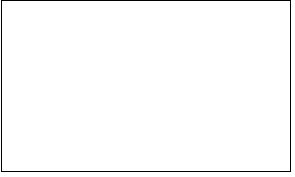
\includegraphics{figs/grabs.pdf}
%\end{graphicalabstract}
%
%\begin{highlights}
%\item Research highlights item 1
%\item Research highlights item 2
%\item Research highlights item 3
%\end{highlights}

\begin{keywords}
quadrupole exciton \sep polariton \sep \WGM \sep \BEC
\end{keywords}


\maketitle

\section{Introdution}

The Internet of Things (IoT) has experienced tremendous growth in recent years, with an ever-increasing number of devices being connected and integrated into various applications, such as smart cities, industrial automation, and environmental monitoring. One key aspect enabling this widespread adoption is Machine Type Communication (MTC), which facilitates seamless communication between machines and devices without human intervention. MTC allows for efficient data exchange among heterogeneous devices, leading to better coordination and improved overall system performance.

In this context, interoperability plays a vital role in ensuring the seamless functioning of IoT ecosystems. As the number and diversity of connected devices continue to grow, so does the need for a robust mechanism to manage communication between devices employing different communication protocols, data formats, and standards. MTC gateways serve as an essential bridge between these devices and the network infrastructure, enabling effective data routing and ensuring smooth communication among heterogeneous devices.

Existing MTC gateway implementations predominantly rely on high-level programming languages, which offer the advantages of rapid development cycles and ease of use. However, these high-level languages often come with trade-offs, such as limited control over hardware resources, increased memory overhead, and suboptimal performance. These limitations can pose significant challenges when deploying large-scale IoT systems, where efficient resource utilization, interoperability, and high-throughput data transmission are essential.

In this paper, we present a novel MTC gateway implementation using a low-level programming language to address the limitations of high-level language-based implementations. Our approach is designed to deliver superior performance, reduced memory overhead, and increased control over hardware resources, while maintaining compatibility with a wide range of MTC protocols. By focusing on key challenges associated with MTC gateways, such as protocol interoperability, scalability, and latency, our implementation aims to provide a robust and efficient solution for the evolving IoT landscape.

\textcolor{red}{Paper structure}
The remainder of this paper is organized as follows: Section 2 provides a comprehensive review of the related work in MTC gateway implementations, discussing various programming languages and architectural choices, as well as the importance of interoperability in IoT systems. Section 3 delves into the specific challenges associated with MTC protocol integration and outlines the design principles of our novel low-level language-based gateway. Section 4 presents the experimental setup and performance evaluation of our proposed solution. Finally, Section 5 concludes the paper and highlights potential future research directions.

\section{Related work}

Machine-Type Communication (MTC) has become an increasingly critical aspect of modern communication systems, driving the transformation of various applications in the ever-evolving Internet of Things (IoT) ecosystem. MTC enables the seamless interaction between a vast array of devices, ranging from wearables and smartphones to industrial equipment and smart home appliances, facilitating the data exchange required for intelligent and automated decision-making processes. With the exponential growth of IoT devices and their stringent requirements for low latency, high reliability, and energy efficiency, the implementation of MTC in low-level languages has emerged as a promising solution to address these challenges.

In this section, we will provide an overview of the current state-of-the-art in MTC gateway implementations, highlighting the advantages and disadvantages of various programming languages and architectural choices. Additionally, we will explore the specific challenges associated with MTC protocol integration and discuss how our novel approach addresses these issues to provide a comprehensive solution for the next generation of IoT deployments.

Rubi et al. \cite{Rubi2019} propose an IoMT platform with a cloud-based electronic health system that collects data from various sources and relays it through gateways or fog servers. The platform enables data management, visualization of electronic records, and knowledge extraction through big data processing, machine learning, and online analytics processing. Additionally, it offers data sharing services for third-party applications, improving healthcare services and interoperability.

The authors in \cite{Volkov2017} conducted IoTDM service testing for smart city management, focusing on the ecological situation in Saint-Petersburg's central district, using an SDN network infrastructure. They developed a hierarchical model and IoT traffic generator in compliance with oneM2M specifications and implemented HTTP, CoAP, and MQTT protocols. Their findings suggested that HTTP is the most suitable protocol for registering IoT devices to the IoTDM service, while MQTT is optimal for transmitting sensor data. The authors concluded that the SDN approach significantly reduces the RTT parameter, demonstrating its potential in managing IoT traffic in smart city environments.

Soumya et al. \cite{Datta2015} explore Fog Computing as a consumer-centric IoT service deployment platform, particularly for connected vehicles and intelligent transportation systems requiring low latency, high mobility, real-time data analytics, and wide geographic coverage. They present an IoT architecture for connected vehicles, integrating Fog Computing platforms into oneM2M standard architecture. The architecture comprises virtual sensing zones, Access Points (RSUs), M2M gateways, and cloud systems. Fog Computing enables consumer-centric services such as M2M data analytics with semantics, discovery of IoT services, and management of connected vehicles. The paper highlights the advantages of Fog Computing, including reduced latency, improved QoS, real-time data analysis, and actuation for superior user experience and consumer-centric IoT products.

This paper \cite{Liang2018} presents a cluster-based congestion-mitigating access scheme (CCAS) that addresses the issue of collision and access efficiency in machine-to-machine (M2M) communications. The authors propose a modified spectral clustering algorithm to form clusters based on the location and service requirements of machine-type communication devices (MTCDs), ensuring that devices with similar requirements are grouped together. They also develop an MTCG (machine-type communication gateway) selection algorithm that considers the delay requirements of MTCDs and selects an MTCG with the appropriate forwarding threshold. The proposed CCAS divides the data transmission process into an MTCD-MTCG stage and an MTCG-BS (base station) stage to reduce collision probability and increase the number of successfully received packets, without causing additional average access delays for MTCDs. The paper includes a theoretical analysis of the MTCG aggregation and forwarding process, as well as performance evaluations through simulations.

% https://www.scopus.com/results/results.uri?sort=plf-f&src=s&st1=%28onem2m+OR+mtc%29+and+%22API%22&sid=2e6f61fce202fa9e6635e553544fee3c&sot=b&sdt=b&sl=40&s=TITLE-ABS-KEY%28%28onem2m+OR+mtc%29+and+%22API%22%29&origin=searchbasic&editSaveS=&yearFrom=Before+1960&yearTo=Present

\printcredits

%% Loading bibliography style file
%\bibliographystyle{model1-num-names}
%\bibliographystyle{cas-model2-names}
\bibliographystyle{unsrt} % Estilo de Bibliografia
% Loading bibliography database
\bibliography{cas-refs}


%\vskip3pt

\bio{figs/bioFig}
My name is Rafael Pereira, I'm 22 years old, and I'm an MSc Computer Engineering Student and Researcher at Polytechnic of Leiria. I'm extremely curious about the technology world, ambitious for knowledge in this area, I'm dedicated to doing my work. The programming thing always got me, and every day it grows. Today I'm looking for interesting projects, that can make me think and learn every day.
\endbio

\end{document}
